\scanpage{45}
\figure{
\begin{tikzpicture}[x=.35cm,y=.35cm]
\draw[line width=1.2pt] (3.0,8.6)--(3.15,9.15);
\fill (3.22,9.37) circle (.08); \fill (3.51,9.56) circle (.12);
\fill (5.37,8.03) circle (.13); \fill (5.30,7.79) circle (.08);
\draw[line width=1.3pt] (5.18,7.25)--(5.10,6.88);\draw[line width=1.8pt] (5.08,6.69)--(5.02,6.51);
\draw[line width=2.4pt] (3.30,6.77)--(3.11,6.04)--(3.04,5.68);
\draw[line width=1.1pt] (2.57,6.06)--(2.49,5.35);\fill (2.63,6.27) circle (.12);\fill (3.04,4.96) circle (.10);
\draw[line width=1.3pt] (4.76,5.35)--(4.70,4.74)--(4.64,4.53);
\fill (.57,4.34) circle (.09);\fill (.48,3.95) circle (.08);
\draw[line width=2.2pt] (.69,3.79) .. controls (.73,3.29) and (.60,3.13) .. (.56,2.98);
\foreach \x/\y in {.31/3.43,.24/3.20,.20/2.93,.14/2.75,.13/2.53,.14/2.33,.26/2.12,.34/1.91} {\fill (\x,\y) circle (.07);}
\draw[line width=1.7pt] (.38,2.73) .. controls (.34,1.90) and (.69,1.41) .. (1.28,1.25);
\fill (1.18,1.27) ellipse (.17 and .11);\fill (1.98,1.39) ellipse (.14 and .09);
\draw[line width=1.7pt] (2.43,2.67) .. controls (2.92,2.18) and (3.67,2.39) .. (4.33,2.94);
\fill (2.21,3.03) ellipse (.11 and .17);
\end{tikzpicture}}
\uline{Cristaux}
\margin{\illegible{1}\quad \unsure{C}\illegible{1}\quad \unsure{C}\illegible{1}\unsure{n}\quad \illegible{1}\quad \unsure{C}\illegible{1}\unsure{n}\quad \unsure{C}\illegible{1}\unsure{on}}

Soit $J$ un idéal principal d'un anneau $A$, $J=\pi A$. Formellement, pour y définir des puissances divisées, on est amené à définir des
\[
\frac{(\pi y)^n}{n!}=\frac{\pi^n}{n!}y^n=\pi^{(n)}y^n
\]
\margin{\illegible{1}\quad \unsure{C}\illegible{1}\quad \illegible{1}\quad \unsure{Canson|CANSON}\quad \illegible{1}\quad \unsure{Canson|CANSON}}
donc à définir des éléments
\[
\pi^{(0)}=1\qquad\deleted{\unsure{et}}\quad\pi^{(n)}\in\pi A\qquad(n\geq1)
\]
qui satisfassent aux conditions suivantes.
\margin{\unsure{Canson|CANSON}\quad \unsure{Canson|CANSON}\quad \unsure{C}\illegible{1}\unsure{n}\quad \unsure{Canson|CANSON}\quad \unsure{C}\illegible{1}\unsure{n}\quad \unsure{Canson|CANSON}}
\figure{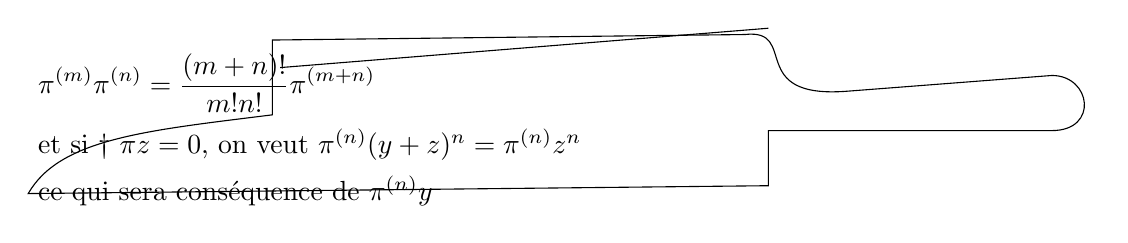
\begin{tikzpicture}[x=1cm,y=1cm]
\node[anchor=north west,text width=13cm,align=left] at (0,0) {\deleted{$\displaystyle\pi^{(m)}\pi^{(n)}=\frac{(m+n)!}{m!n!}\pi^{(m+n)}$}\\[5pt]\deleted{et si $\unsure{\dagger}$ $\pi z=0$, on veut $\pi^{(n)}(y+z)^n=\pi^{(n)}z^n$}\\[5pt]\deleted{ce qui sera conséquence de $\pi^{(n)}y$}};
\draw (3.1,.05)--(9.1,.12) .. controls (9.8,.2) and (9.1,-.7) .. (10.4,-.6)--(13,-.4) .. controls (13.5,-.4) and (13.6,-1.1) .. (13,-1.1)--(9.4,-1.1)--(9.4,-1.8)--(0,-1.9) .. controls (.4,-1.2) and (1.5,-1.1) .. (3.1,-.9)--cycle;
\draw (3.2,-.3)--(9.4,.2);
\end{tikzpicture}}
\[
\pi^{(1)}=\pi
\]
\margin{\unsure{Canson|CANSON}\quad \unsure{C}\illegible{1}\quad \illegible{1}\quad \illegible{1}\quad \unsure{Canson|CANSON}\quad \unsure{Canson|CANSON}}
\[
\unsure{\alpha|a}\quad\left\{\begin{aligned}
\pi^{(m)}\pi^{(n)}&=\frac{\unsure{(m+n)!|(m+n!}}{m!n!}\pi^{(m+n)}\\
\pi^{(p)}\left(\frac{\pi^{(q)}}{\pi}\right)^p&=\frac{(pq)!}{p!(q!)^p}\pi^{(pq)}.
\end{aligned}\right.
\]
\uline{NB} Comme $\pi^{(q)}\in\pi A$, $\dfrac{\pi^{(q)}}{\pi}$ est défini mod. addition d'un $z$ tel que $\pi z=0$, mais comme $\pi^{(p)}\in\pi A$, on détermine sans ambiguïté l'élément $\pi^{(p)}\left(\dfrac{\pi^{(q)}}{\pi}\right)^p$.

\margin{\illegible{1}\unsure{on}\quad \illegible{1}\quad \illegible{1}\unsure{n}\quad \illegible{1}\unsure{n}\quad \illegible{1}\unsure{on}\quad \unsure{C}\illegible{1}\unsure{on}}

Alors on trouve une structure de puissances divisées \inserted{de $I=\pi A$} en posant
\[
x^{(n)}=(\pi y)^{(n)}=\pi^{(n)}y^n\qquad\text{pour }x=\pi y\in J,
\]
\margin{\illegible{1}\unsure{on}\quad \unsure{Canson|CANSON}\quad \unsure{Canson|CANSON}\quad \unsure{C}\illegible{1}\quad \unsure{C}\illegible{1}\unsure{on}\quad \illegible{1}\unsure{on}}
en notant que $x^{(n)}$ ne dépend pas du choix de $y$ \unsure{t.q.|d.q.} $x=\pi y$.

\uline{Exemple$^1$} Supposons que $A$ soit sans torsion sur $\mathbb Z$. Alors les \deleted{\unsure{premières}} relations
\[
\pi^n=n!\pi^{(n)}
\]
\margin{\illegible{1}\quad \illegible{1}\quad \illegible{1}\quad \unsure{C}\illegible{1}}
déterminent uniquement les $\pi^{(n)}$ en fonction de $\pi$, et leur existence équivaut au fait que $\pi^n\in n!A\quad\forall n\geq2$. Les relations $\unsure{\alpha|a}$ sont satisfaites automatiquement.

\uline{Exemple$^2$} Supposons $A_o=\mathbb Z_{(p\mathbb Z)}$, \deleted{Alors} $\pi=p$. Alors les conditions précédentes sont satisfaites,
\margin{\unsure{Canson|CANSON}\quad \unsure{C}\illegible{1}\unsure{on}\quad \illegible{1}\quad \unsure{C}\illegible{1}\quad \illegible{1}}
les $\dfrac{p^n}{n!}$ sont des entiers p-adiques. Donc si $A$ est un anneau dans lequel tout nb premier $q\ne p$ est inv. (i.e. les seules car. résiduelles sont $p,0$), \unsure{i.e.} une algèbre sur $A_o$, on trouve par spécialisation des $\pi^{(n)}\in A$, $\pi^{(n)}=\dfrac{p^n}{n!}$, qui
\margin{\illegible{1}\quad \illegible{1}\quad \illegible{1}}
\mspage{44}
